\documentclass[12pt, a4paper, oneside]{book}

% ===========================================
% PAQUETES NECESARIOS
% ===========================================
\usepackage[utf8]{inputenc}
\usepackage[spanish]{babel}
\usepackage{amsmath, amssymb, amsfonts}
\usepackage{graphicx}
\usepackage{geometry}
\usepackage{fancyhdr}
\usepackage{xcolor}
\usepackage{listings}
\usepackage{hyperref}
\usepackage{booktabs}
\usepackage{array}
\usepackage{titlesec}
\usepackage{enumitem}
\usepackage{tikz}
\usepackage{amsthm}

% ===========================================
% CONFIGURACIÓN DE PÁGINA
% ===========================================
\geometry{
  left=3cm,
  right=2.5cm,
  top=2.5cm,
  bottom=2.5cm
}

% ===========================================
% CONFIGURACIÓN DE ENCABEZADOS
% ===========================================
\pagestyle{fancy}
\fancyhf{}
\rhead{\leftmark}           % Título del capítulo
\lhead{Funciones Matemáticas} % Título general (personalizable)
\cfoot{\thepage}
\renewcommand{\headrulewidth}{0.4pt}

% ===========================================
% CONFIGURACIÓN DE TÍTULOS
% ===========================================
\titleformat{\chapter}[display]
  {\normalfont\bfseries\centering}{\chaptertitlename\ \thechapter}{20pt}{\Huge}

% ===========================================
% ENTORNOS MATEMÁTICOS (UNIFICADOS)
% ===========================================
\theoremstyle{definition}
\newtheorem{definicion}{Definición}[chapter]
\newtheorem{teorema}{Teorema}[chapter]
\newtheorem{proposicion}{Proposición}[chapter]
\newtheorem{ejemplo}{Ejemplo}[chapter]
\newtheorem{ejercicio}{Ejercicio}[chapter]

% ===========================================
% CONFIGURACIÓN DE CÓDIGO (LINGO)
% ===========================================
\lstset{
    language=C,
    basicstyle=\ttfamily\footnotesize,
    backgroundcolor=\color{white},
    frame=single,
    breaklines=true,
    showstringspaces=false,
    numbers=left,
    numberstyle=\tiny\color{gray},
    keywordstyle=\color{black}\bfseries,
    commentstyle=\color{gray},
    stringstyle=\color{black}
}

% ===========================================
% CONFIGURACIÓN DE HIPERVÍNCULOS
% ===========================================
\hypersetup{
  pdftitle={Informe de Programación Lineal},
  pdfauthor={Jefry Erick Quispe Ramos},
  pdfsubject={Problemas con Solver y Lingo},
  colorlinks=true,
  linkcolor=black,
  urlcolor=black,
  citecolor=black
}

% ===========================================
% COMANDO PARA LA PORTADA
% ===========================================
\newcommand{\portada}{
  \begin{titlepage}
    \centering
    {\scshape\LARGE Universidad Nacional del Altiplano\par}
    \vspace{1.5cm}
    {\scshape\Large Problemas resueltos con diferentes métodos\par}
    \vspace{1.5cm}
    {\huge\bfseries Informe de Investigacion de Operaciones\par}
    \vspace{2cm}
    {\Large Presentado por:\par}
    \vspace{0.5cm}
    {\Large Jefry Erick Quispe Ramos\\
    Nestor Ademir Ruelas Yana}
    \vfill
    {\large \today\par}
  \end{titlepage}
}

% ===========================================
% INICIO DEL DOCUMENTO
% ===========================================
\begin{document}

\portada
\tableofcontents
\newpage

% ===========================================
% EJERCICIO 1: ASIGNACIÓN DE NADADORAS
% ===========================================

\chapter{PROGRAMACION LINEAL}

\section{DEFINICIONES}

\begin{definicion}[Programación Lineal (PL)]
Modelo matemático para optimizar (maximizar o minimizar) una función objetivo lineal, sujeta a restricciones lineales de igualdad o desigualdad. Todos las variables son continuas.

\textbf{Ejemplo estándar:}
\begin{align*}
\text{Maximizar } & \mathbf{c}^T\mathbf{x} \\
\text{sujeto a } & A\mathbf{x} \leq \mathbf{b} \\
& \mathbf{x} \geq 0
\end{align*}
\end{definicion}

\begin{definicion}[Programación Lineal Entera (PLE)]
Variante de PL donde \textbf{todas las variables} deben tomar valores enteros. Esencial para problemas discretos (ej: asignación de recursos indivisibles).

\textbf{Caso típico:}
\begin{equation*}
x_i \in \mathbb{Z}^+ \quad \forall i
\end{equation*}
\end{definicion}

\begin{definicion}[Programación Lineal Mixta (PLM)]
Combina variables continuas y enteras en un mismo modelo. Usada cuando solo algunas decisiones requieren discretización.

\textbf{Estructura:}
\begin{equation*}
\begin{cases}
x_1, x_2 \in \mathbb{R}^+ \\
x_3 \in \{0,1\} \quad \text{(variable binaria)}
\end{cases}
\end{equation*}
\end{definicion}

\begin{definicion}[Solución con Solver]
Herramienta de Excel para PL/PLM. Requiere:
\begin{itemize}[leftmargin=*]
\item Definir celda objetivo
\item Especificar variables de decisión
\item Añadir restricciones mediante interfaz gráfica
\end{itemize}

\textbf{Ventaja:} Accesible sin necesidad de código.
\end{definicion}

\begin{definicion}[Modelado en LINGO]
Lenguaje especializado para optimización. Sintaxis compacta y eficiente para problemas grandes.

\textbf{Ejemplo básico en LINGO:}
\begin{lstlisting}[language=C]
MODEL:
    MAX = 20*x1 + 30*x2;
    x1 <= 50;       ! Restricción capacidad;
    x2 <= 60;
    x1 + 2*x2 <= 120;
    @GIN(x1);       ! Variable entera;
END
\end{lstlisting}

\textbf{Comandos clave:}
\begin{itemize}[leftmargin=*]
\item \texttt{@GIN(x)}: Variable entera
\item \texttt{@BIN(x)}: Variable binaria (0/1)
\item \texttt{@FREE(x)}: Variable no restringida
\end{itemize}
\end{definicion}

\section{EJERCICIO 1: Programacion entera con solver: Competencia de natacion}

Para una competencia de relevos 4x100 metros, un equipo de natación debe asignar a cada nadadora uno de los cuatro estilos: libre, pecho, mariposa y dorso. El objetivo es asignar a cada nadadora un estilo de manera que se minimice el tiempo total del equipo. Este problema se resuelve mediante \textbf{programación lineal entera} utilizando \textbf{Excel Solver}.

\subsection{2. Datos del problema}

Los tiempos (en segundos) que cada nadadora tarda en nadar cada estilo son los siguientes:

\begin{center}
\begin{tabular}{lcccc}
\toprule
\textbf{Nadadora} & \textbf{Libre} & \textbf{Pecho} & \textbf{Mariposa} & \textbf{Dorso} \\
\midrule
Gabriela Hernández & 54 & 54 & 51 & 53 \\
Marcela Salinas     & 51 & 57 & 52 & 52 \\
Julia Martínez      & 50 & 53 & 54 & 56 \\
Claudia Gómez       & 56 & 54 & 55 & 53 \\
\bottomrule
\end{tabular}
\end{center}

\subsection{3. Formulación del modelo}

\subsection{Variables de decisión}

Sea $X_{ij} = 
\begin{cases}
1 & \text{si la nadadora } i \text{ nada el estilo } j \\
0 & \text{en otro caso}
\end{cases}$

donde \( i \in \{1,2,3,4\} \) representa a cada nadadora y \( j \in \{1,2,3,4\} \) a cada estilo (Libre, Pecho, Mariposa, Dorso).

\subsection{Función objetivo}

Minimizar el tiempo total:

\[
\min Z = \sum_{i=1}^{4} \sum_{j=1}^{4} c_{ij} X_{ij}
\]

Donde \( c_{ij} \) es el tiempo que la nadadora \( i \) tarda en el estilo \( j \).

En este caso:

\[
\min Z = 54X_{11} + 54X_{12} + 51X_{13} + 53X_{14} + 
51X_{21} + 57X_{22} + 52X_{23} + 52X_{24} +
50X_{31} + 53X_{32} + 54X_{33} + 56X_{34} +
56X_{41} + 54X_{42} + 55X_{43} + 53X_{44}
\]

\subsection{Restricciones}

\begin{itemize}
    \item Cada estilo debe ser asignado a una sola nadadora:
    \[
    \sum_{i=1}^{4} X_{ij} = 1 \quad \text{para todo } j = 1,2,3,4
    \]

    \item Cada nadadora debe nadar un solo estilo:
    \[
    \sum_{j=1}^{4} X_{ij} = 1 \quad \text{para todo } i = 1,2,3,4
    \]

    \item Variables binarias:
    \[
    X_{ij} \in \{0,1\} \quad \text{para todo } i,j
    \]
\end{itemize}

\subsection{4. Resolución con Excel Solver}

Se utilizó Excel Solver para encontrar la combinación óptima. Las variables \( X_{ij} \) se modelaron como celdas binarias (0 o 1). La función objetivo fue el \texttt{=SUMAPRODUCTO(tiempos, decisiones)}.


\begin{center}
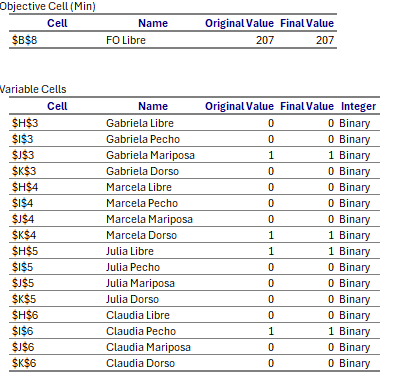
\includegraphics[width=0.8\textwidth]{fotos/Solverfinal.png}
\end{center}

\subsection{5. Solución óptima}

La asignación óptima es:

\begin{itemize}
    \item Gabriela: Mariposa
    \item Marcela: Dorso
    \item Julia: Libre
    \item Claudia: Pecho
\end{itemize}

Tiempo total mínimo: \textbf{207 segundos}.

\newpage
\section{Ejercicio 2: Progamacion entera : Fabricación de lotes de prendas (Programación Lineal Entera Mixta)}

Se planteó un modelo de programación lineal para maximizar las ganancias en la producción de dos tipos de extractos: para beber y concentrado. El modelo fue resuelto utilizando el complemento \textbf{Solver de Excel}, obteniéndose una solución óptima.

\textbf{Datos del problema:}

\begin{center}
\begin{tabular}{|l|c|c|c|}
\hline
\textbf{Parámetro} & \textbf{Pantalones} & \textbf{Chalecos} & \textbf{Chamarras} \\
\hline
Piel por unidad (pies$^2$) & 5 & 3 & 8 \\
Mano de obra por unidad (h) & 4 & 3 & 5 \\
Costo variable por unidad (\$) & 30 & 20 & 80 \\
Costo fijo por lote (\$) & 100 & 80 & 150 \\
Precio de venta (\$) & 60 & 40 & 120 \\
Producción mínima si se fabrica & 100 & 150 & 200 \\
\hline
\end{tabular}
\end{center}

Disponibilidades:
\begin{itemize}
    \item Piel disponible: 3000 pies$^2$
    \item Mano de obra disponible: 2500 horas
\end{itemize}

\subsection{Modelo matemático}

\textbf{Variables:}
\begin{itemize}
    \item $x_i$: unidades a fabricar del producto $i$
    \item $y_i$: variable binaria, vale 1 si se fabrica el producto $i$, 0 si no
\end{itemize}

\textbf{Función objetivo:}
\[
\max Z = \sum_{i=1}^{3} \left[ (PV_i - CVAR_i)\cdot x_i - CFIJO_i \cdot y_i \right]
\]

\textbf{Restricciones:}
\begin{align*}
5x_1 + 3x_2 + 8x_3 &\leq 3000 && \text{(restricción de piel)} \\
4x_1 + 3x_2 + 5x_3 &\leq 2500 && \text{(restricción de mano de obra)} \\
x_1 &\leq 999999 y_1 \\
x_2 &\leq 999999 y_2 \\
x_3 &\leq 999999 y_3 \\
x_1 &\geq 100 y_1 \\
x_2 &\geq 150 y_2 \\
x_3 &\geq 200 y_3 \\
x_i &\in \mathbb{Z}_{\geq 0},\quad y_i \in \{0,1\} && \text{(enteras y binarias)}
\end{align*}

\subsection{Solución óptima}

\begin{center}
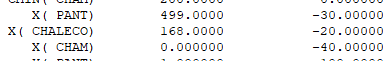
\includegraphics[width=0.5\textwidth]{fotos/ejercicio2.png}
\end{center}

Según LINGO, la solución óptima es:

\begin{itemize}
    \item \textbf{Pantalones:} 499 unidades ($y_1 = 1$)
    \item \textbf{Chalecos:} 168 unidades ($y_2 = 1$)
    \item \textbf{Chamarras:} 0 unidades ($y_3 = 0$)
\end{itemize}

\textbf{Utilidad total:} \$18,150

Esto significa que se deben fabricar pantalones y chalecos, y no conviene fabricar chamarras en este caso.

\newpage
\subsection{Código LINGO usado}

\begin{verbatim}
SETS:
PRODUCTO /Pant, Chaleco, Cham/ : PIEL, MOBRA, CVAR, CFIJO, PV, CMIN, X, Y;
ENDSETS

DATA:
PIEL   = 5 3 8;
MOBRA  = 4 3 5;
CVAR   = 30 20 80;
CFIJO  = 100 80 150;
PV     = 60 40 120;
CMIN   = 100 150 200;
ENDDATA

! Función objetivo:
MAX = @SUM(PRODUCTO(I): (PV(I) - CVAR(I))*X(I) - CFIJO(I)*Y(I));

! Restricciones:
@SUM(PRODUCTO(I): PIEL(I)*X(I)) <= 3000;
@SUM(PRODUCTO(I): MOBRA(I)*X(I)) <= 2500;

@FOR(PRODUCTO(I): X(I) <= 999999*Y(I));
@FOR(PRODUCTO(I): X(I) >= CMIN(I)*Y(I));

@FOR(PRODUCTO(I): @BIN(Y(I)));
@FOR(PRODUCTO(I): @GIN(X(I)));
\end{verbatim}


\newpage

\section{EJERCICIO 3: Programacion entera: Fabricacion de articulos}

Un empresario que fabrica tres artículos \(P_1, P_2, P_3\), desea encontrar la producción diaria que le permita maximizar sus beneficios. Los artículos son procesados en dos de las cuatro máquinas disponibles, ya sea en A y B, o bien en C y D. Los costos diarios fijos por iniciar estas máquinas son:

\begin{itemize}
    \item Máquina A: 20 unidades monetarias,
    \item Máquina B: 25 unidades monetarias,
    \item Máquina C: 35 unidades monetarias,
    \item Máquina D: 15 unidades monetarias.
\end{itemize}

Los ingresos por unidad vendida son:

\begin{itemize}
    \item \(P_1\): 5 unidades monetarias,
    \item \(P_2\): 5 unidades monetarias,
    \item \(P_3\): 10 unidades monetarias.
\end{itemize}

Las horas necesarias para procesar una unidad de cada artículo en cada máquina se muestran en la siguiente tabla:

\begin{center}
\begin{tabular}{|c|c|c|c|c|}
\hline
 & A & B & C & D \\
\hline
P1 & 1 & 1 & 2 & 1 \\
P2 & 1 & 1 & 1 & 2 \\
P3 & 2 & 1 & 1 & 1 \\
\hline
\end{tabular}
\end{center}

Las horas disponibles por día en las máquinas son:  
Máquina A: 190 h, B: 210 h, C: 170 h, D: 200 h.

\subsection{Definición de variables}

\begin{itemize}
    \item \(x_1, x_2, x_3\): número de unidades producidas de \(P_1, P_2, P_3\), respectivamente.
    \item \(y_1 = 1\) si se utilizan las máquinas A y B, 0 en otro caso.
    \item \(y_2 = 1\) si se utilizan las máquinas C y D, 0 en otro caso.
\end{itemize}

\subsection{Función Objetivo}

\[
\text{Maximizar } Z = 5x_1 + 5x_2 + 10x_3 - \left[ (20 + 25)y_1 + (35 + 15)y_2 \right]
\]

\subsection{Restricciones}

\begin{align*}
x_1 + x_2 + 2x_3 &\leq 190 + M(1 - y_1) \quad &\text{(Máquina A)} \\
x_1 + x_2 + x_3 &\leq 210 + M(1 - y_1) \quad &\text{(Máquina B)} \\
2x_1 + x_2 + x_3 &\leq 170 + M(1 - y_2) \quad &\text{(Máquina C)} \\
x_1 + 2x_2 + x_3 &\leq 200 + M(1 - y_2) \quad &\text{(Máquina D)} \\
y_1 + y_2 &= 1 \\
x_1, x_2, x_3 &\geq 0,\quad \text{enteras} \\
y_1, y_2 &\in \{0,1\}
\end{align*}

\subsection{Resolución por Enumeración de Casos}

\subsection{Caso 1: \(y_1 = 1, y_2 = 0\)}

Se utilizan máquinas A y B.  
\[
Z = 5x_1 + 5x_2 + 10x_3 - 45
\]
\[
\begin{aligned}
x_1 + x_2 + 2x_3 &\leq 190 \\
x_1 + x_2 + x_3 &\leq 210
\end{aligned}
\]

Maximizamos \(x_3\), pues tiene mayor contribución. Si \(x_3 = 95\), entonces:

\[
x_1 = x_2 = 0 \Rightarrow Z = 950 - 45 = 905
\]

\subsection{Caso 2: \(y_1 = 0, y_2 = 1\)}

Se utilizan máquinas C y D.  
\[
Z = 5x_1 + 5x_2 + 10x_3 - 50
\]
\[
\begin{aligned}
2x_1 + x_2 + x_3 &\leq 170 \\
x_1 + 2x_2 + x_3 &\leq 200
\end{aligned}
\]

Probamos \(x_3 = 90, x_1 = 0, x_2 = 40\):

\[
2(0) + 40 + 90 = 130 \leq 170 \\
0 + 80 + 90 = 170 \leq 200
\]

Entonces:  
\[
Z = 5(0) + 5(40) + 10(90) - 50 = 1050
\]

\subsection{Conclusión}

La mejor alternativa es utilizar las máquinas C y D, con la siguiente producción:

\[
x_1 = 0, \quad x_2 = 40, \quad x_3 = 90
\]

El beneficio máximo es:
\[
\boxed{Z = 1050}
\]


\newpage
\section{Ejercicio 4: programacion lineal con lingo: Mercado}

Una cierta empresa tiene una sola línea de producción en la cual tiene que producir los tres productos (A, B y C) que mantiene en el mercado. Las demandas diarias que tiene que satisfacer para la siguiente semana, los ritmos de producción, los inventarios iniciales y los costos diarios de inventario por unidad de cada producto son los siguientes:

\begin{center}
\begin{tabular}{|c|cccccc|c|c|c|}
\hline
\textbf{Producto} & \textbf{Día 1} & \textbf{Día 2} & \textbf{Día 3} & \textbf{Día 4} & \textbf{Día 5} & \textbf{Día 6} & \textbf{Ritmo (unid/hora)} & \textbf{Inventario inicial} & \textbf{Costo inventario} \\
\hline
A & 45 & 30 & 35 & 25 & 30 & 35 & 10 & 60 & 3 \\
B & 15 & 10 & 15 & 20 & 15 & 15 & 15 & 0 & 2 \\
C & 20 & 25 & 30 & 25 & 25 & 30 & 20 & 10 & 2 \\
\hline
\end{tabular}
\end{center}

La línea de producción tiene una capacidad diaria de 16 horas, pero por cada tipo de producto que se decida fabricar en el día se consumen 2 horas adicionales por preparación. El costo de cada preparación es de \$150.

Se desea programar la producción para los seis días de la semana, cumpliendo toda la demanda y minimizando la suma total de los costos de inventario y de preparación.

\subsection{Variables}

\begin{itemize}
    \item \(x_{i,j}\): unidades del producto \(i\) producidas en el día \(j\),
    \item \(inv_{i,j}\): inventario del producto \(i\) al final del día \(j\),
    \item \(z_{i,j}\): variable binaria que indica si el producto \(i\) fue producido el día \(j\) (1) o no (0).
\end{itemize}

\subsection{Función Objetivo}

Minimizar el costo total:
\[
\min \sum_{i=1}^{3} \sum_{j=1}^{6} 150 \cdot z_{i,j} + inv_{i,j} \cdot \text{costo\_inv}_i
\]

\subsection{Restricciones}

\begin{itemize}
    \item Inventario inicial:
    \[
    inv_{i,1} = x_{i,1} + \text{inv\_inicial}_i - \text{demanda}_{i,1}
    \]
    \item Balance de inventario para días siguientes:
    \[
    inv_{i,j} = inv_{i,j-1} + x_{i,j} - \text{demanda}_{i,j} \quad \forall j = 2, \dots, 6
    \]
    \item Límite de producción diaria:
    \[
    \sum_{i=1}^{3} \frac{x_{i,j}}{\text{ritmo}_i} + 2 \cdot \sum_{i=1}^{3} z_{i,j} \leq 16 \quad \forall j
    \]
    \item Relación entre producción y preparación:
    \[
    x_{i,j} \leq M \cdot z_{i,j}
    \]
    Donde \(M\) es un número suficientemente grande.
\end{itemize}

\subsection{Código LINGO}

\begin{verbatim}
sets:
  prod/1..3/: inv_inicial, costo_inv, ritmo;
  dia/1..6/;
  pd(prod, dia): demanda, inv, x, z;
endsets

data:
  inv_inicial = 60 0 10;
  costo_inv = 3 2 2;
  ritmo = 10 15 20;
  demanda =
    45 30 35 25 30 35
    15 10 15 20 15 15
    20 25 30 25 25 30;
enddata

min = @sum(pd(i,j): 150 * z(i,j) + inv(i,j) * costo_inv(i));

@for(pd(i,j): x(i,j) <= 1000 * z(i,j));
@for(dia(j): @sum(prod(i): x(i,j)/ritmo(i)) + 2 * @sum(prod(i): z(i,j)) <= 16);
@for(prod(i): inv_inicial(i) + x(i,1) = demanda(i,1) + inv(i,1));
@for(pd(i,j) | j #ge# 2: inv(i,j-1) + x(i,j) = demanda(i,j) + inv(i,j));
@for(pd(i,j): @bin(z(i,j)));
\end{verbatim}

\subsection{Resultado LINGO}

\begin{center}
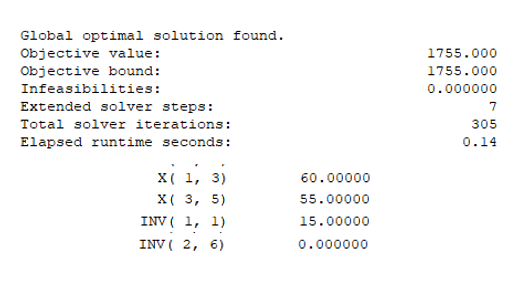
\includegraphics[width=0.95\textwidth]{fotos/eje4.png}
\end{center}

\subsection{Resultados}

\subsection{Solución Óptima}
El solver LINGO encontró una solución óptima global con un \textbf{costo total mínimo de \$1,755}. A continuación se detallan los resultados clave:

\begin{itemize}
    \item \textbf{Tipo de modelo}: Programación Lineal Entera Mixta (MILP).
    \item \textbf{Variables enteras}: 18 (preparaciones $z_{i,j}$).
    \item \textbf{Tiempo de ejecución}: 0.14 segundos.
\end{itemize}

\subsection{Producción por Día}
\begin{table}[h!]
\centering
\caption{Producción óptima ($x_{i,j}$) y preparaciones ($z_{i,j}$)}
\begin{tabular}{|c|c|c|c|c|c|c|}
\hline
\textbf{Producto} & \textbf{Día 1} & \textbf{Día 2} & \textbf{Día 3} & \textbf{Día 4} & \textbf{Día 5} & \textbf{Día 6} \\ \hline
A & 0 (0) & 15 (1) & 60 (1) & 0 (0) & 65 (1) & 0 (0) \\ \hline
B & 40 (1) & 0 (0) & 0 (0) & 50 (1) & 0 (0) & 0 (0) \\ \hline
C & 35 (1) & 0 (0) & 55 (1) & 0 (0) & 55 (1) & 0 (0) \\ \hline
\end{tabular}
\label{tab:produccion}
\end{table}
\textit{Nota: Valores en formato "unidades (preparación)". 1 = preparación activa, 0 = no activa.}

\subsection{Inventarios Finales}
Los inventarios al final de cada día fueron:
\begin{itemize}
    \item \textbf{Producto A}: 15 (Día 1), 0 (Día 2), 25 (Día 3), 0 (Día 4), 35 (Día 5), 0 (Día 6).
    \item \textbf{Producto B}: 25, 15, 0, 30, 15, 0.
    \item \textbf{Producto C}: 25, 0, 25, 0, 30, 0.
\end{itemize}

\subsection{Análisis de Restricciones}
\begin{itemize}
    \item \textbf{Capacidad diaria}: Las restricciones de capacidad fueron activas ($\text{Slack} = 0$) en los días 1, 3 y 5.
    \item \textbf{Preparaciones}: Total de 11 preparaciones activas (costos: \$150 c/u).
\end{itemize}

\newpage
\section{EJERCICIO 5: prog lineal con lingo: Transporte}

Una empresa desea programar el transporte de su producto principal que se elabora en 4 plantas con destino a 3 almacenes. Se conoce la demanda de los almacenes, la capacidad de producción de las plantas y el costo de transporte por unidad de transporte de una planta a un almacén.

\subsection{Datos del Problema}

\textbf{Costos de Transporte (\$/Unidad):}

\begin{center}
\begin{tabular}{|c|c|c|c|c|}
\hline
\textbf{Plantas} & \textbf{Almacén 1} & \textbf{Almacén 2} & \textbf{Almacén 3} & \textbf{Capacidad} \\
\hline
1 & 3 & 2 & 4 & 950 \\
\hline
2 & 2 & 4 & 3 & 1150 \\
\hline
3 & 3 & 5 & 3 & 1000 \\
\hline
4 & 4 & 3 & 2 & 900 \\
\hline
\textbf{Demanda} & \textbf{1200} & \textbf{900} & \textbf{500} & - \\
\hline
\end{tabular}
\end{center}

\textbf{Objetivo:} Elaborar un modelo de programación lineal que permita hallar el plan óptimo de transporte.

\subsection{Definición de Variables}

Sea $x_{ij}$ la cantidad de unidades a transportar desde la planta $i$ hasta el almacén $j$, donde:
\begin{itemize}
    \item $i \in \{1, 2, 3, 4\}$ representa las plantas
    \item $j \in \{1, 2, 3\}$ representa los almacenes
\end{itemize}

$$x_{ij} \geq 0 \quad \forall i \in \{1,2,3,4\}, \forall j \in \{1,2,3\}$$

\subsection{Función Objetivo}

Minimizar el costo total de transporte:

$$\min Z = \sum_{i=1}^{4} \sum_{j=1}^{3} c_{ij} \cdot x_{ij}$$

Donde $c_{ij}$ es el costo unitario de transporte desde la planta $i$ al almacén $j$.

Expandiendo la función objetivo:
\begin{align}
\min Z = &3x_{11} + 2x_{12} + 4x_{13} + 2x_{21} + 4x_{22} + 3x_{23} \nonumber \\
&+ 3x_{31} + 5x_{32} + 3x_{33} + 4x_{41} + 3x_{42} + 2x_{43}
\end{align}

\subsection{Restricciones}

\subsection{Restricciones de Capacidad de las Plantas}
Cada planta no puede enviar más de su capacidad de producción:

\begin{align}
\sum_{j=1}^{3} x_{1j} &\leq 950 \quad \text{(Planta 1)} \\
\sum_{j=1}^{3} x_{2j} &\leq 1150 \quad \text{(Planta 2)} \\
\sum_{j=1}^{3} x_{3j} &\leq 1000 \quad \text{(Planta 3)} \\
\sum_{j=1}^{3} x_{4j} &\leq 900 \quad \text{(Planta 4)}
\end{align}

Equivalentemente:
\begin{align}
x_{11} + x_{12} + x_{13} &\leq 950 \\
x_{21} + x_{22} + x_{23} &\leq 1150 \\
x_{31} + x_{32} + x_{33} &\leq 1000 \\
x_{41} + x_{42} + x_{43} &\leq 900
\end{align}

\subsection{Restricciones de Demanda de los Almacenes}
Cada almacén debe recibir al menos su demanda requerida:

\begin{align}
\sum_{i=1}^{4} x_{i1} &\geq 1200 \quad \text{(Almacén 1)} \\
\sum_{i=1}^{4} x_{i2} &\geq 900 \quad \text{(Almacén 2)} \\
\sum_{i=1}^{4} x_{i3} &\geq 500 \quad \text{(Almacén 3)}
\end{align}

Equivalentemente:
\begin{align}
x_{11} + x_{21} + x_{31} + x_{41} &\geq 1200 \\
x_{12} + x_{22} + x_{32} + x_{42} &\geq 900 \\
x_{13} + x_{23} + x_{33} + x_{43} &\geq 500
\end{align}

\subsection{Restricciones de No Negatividad}
$$x_{ij} \geq 0 \quad \forall i \in \{1,2,3,4\}, \forall j \in \{1,2,3\}$$

\subsection{Verificación de Factibilidad}

\textbf{Capacidad total de las plantas:} $950 + 1150 + 1000 + 900 = 4000$ unidades

\textbf{Demanda total de los almacenes:} $1200 + 900 + 500 = 2600$ unidades

Como la capacidad total (4000) es mayor que la demanda total (2600), el problema es factible y tiene un exceso de capacidad de 1400 unidades.


\subsection{Análisis del Modelo}

Este es un \textbf{problema de transporte desbalanceado} ya que:
\begin{itemize}
    \item Oferta total: 4000 unidades
    \item Demanda total: 2600 unidades
    \item Exceso de oferta: 1400 unidades
\end{itemize}

Al ser un problema con exceso de oferta, algunas plantas no utilizarán toda su capacidad en la solución óptima.

\subsection{Solución Obtenida}

\begin{center}
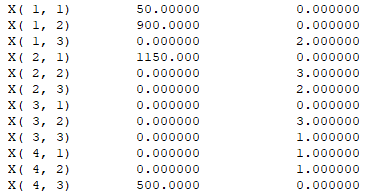
\includegraphics[width=0.95\textwidth]{fotos/eje5.png}
\end{center}


\subsection{Solución Obtenida}

\subsection{Resultados Numéricos}
La solución óptima encontrada por LINGO es:

\begin{table}[h]
\centering
\caption{Asignaciones Óptimas de Transporte ($x_{ij}$)}
\begin{tabular}{|c|c|c|c|}
\hline
\textbf{Planta $\backslash$ Almacén} & \textbf{Almacén 1} & \textbf{Almacén 2} & \textbf{Almacén 3} \\ \hline
Planta 1 & 50 & 900 & 0 \\ \hline
Planta 2 & 1150 & 0 & 0 \\ \hline
Planta 3 & 0 & 0 & 0 \\ \hline
Planta 4 & 0 & 0 & 500 \\ \hline
\end{tabular}
\end{table}

\begin{itemize}
\item \textbf{Costo mínimo total:} \$5,250.00
\item \textbf{Iteraciones del solver:} 4
\item \textbf{Tiempo de ejecución:} 0.06 segundos
\end{itemize}

\subsection{Análisis de Capacidad}
\begin{table}[h]
\centering
\caption{Uso de Capacidad por Planta}
\begin{tabular}{|c|c|c|c|}
\hline
\textbf{Planta} & \textbf{Capacidad Total} & \textbf{Capacidad Usada} & \textbf{Ociosa} \\ \hline
1 & 950 & 950 & 0 \\ \hline
2 & 1150 & 1150 & 0 \\ \hline
3 & 1000 & 0 & 1000 \\ \hline
4 & 900 & 500 & 400 \\ \hline
\end{tabular}
\end{table}

\subsection{Demanda Satisfecha}
\begin{table}[h]
\centering
\caption{Cumplimiento de Demanda}
\begin{tabular}{|c|c|c|}
\hline
\textbf{Almacén} & \textbf{Demanda Requerida} & \textbf{Demanda Cubierta} \\ \hline
1 & 1200 & 1200 (50 + 1150) \\ \hline
2 & 900 & 900 (900) \\ \hline
3 & 500 & 500 (500) \\ \hline
\end{tabular}
\end{table}

\subsection{Interpretación de Resultados}
\begin{itemize}
\item \textbf{Planta 3} no se utiliza en absoluto (totalmente ociosa).
\item \textbf{Planta 4} solo abastece al Almacén 3.
\item La solución aprovecha las rutas más económicas:
  \begin{itemize}
  \item Planta 2 $\rightarrow$ Almacén 1 (costo \$2/unidad)
  \item Planta 1 $\rightarrow$ Almacén 2 (costo \$2/unidad)
  \item Planta 4 $\rightarrow$ Almacén 3 (costo \$2/unidad)
  \end{itemize}
\end{itemize}

\subsection{Resultados Técnicos de LINGO}

\begin{lstlisting}[caption=Parte relevante del output de LINGO]
Global optimal solution found.
Objective value:                              5250.000
Total solver iterations:                             4

Variable           Value
X( 1, 1)        50.00000
X( 1, 2)        900.0000
X( 2, 1)        1150.000
X( 4, 3)        500.0000
\end{lstlisting}


\newpage
\section{EJERCICIO 6: Prog. Lineal: Bloques}

La empresa "Triturados y Derivados S.A." (TRIDESA) desea determinar la cantidad óptima de bloques de concreto tipo I, II y III a producir para maximizar la utilidad, considerando las restricciones de recursos disponibles.

\subsection{Datos del Problema}

\begin{table}[h]
\centering
\begin{tabular}{|c|c|c|c|c|c|c|}
\hline
\textbf{Block} & \textbf{Cemento} & \textbf{Arena} & \textbf{Grava} & \textbf{Agua} & \textbf{H. Máq.} & \textbf{Utilidad} \\
\textbf{(tipo)} & \textbf{(kg)} & \textbf{(kg)} & \textbf{(kg)} & \textbf{(litros)} & \textbf{(horas)} & \textbf{(\$/unidad)} \\
\hline
I & 1.50 & 0.80 & 0.40 & 0.30 & 0.004 & 6 \\
II & 1.20 & 0.60 & 0.60 & 0.40 & 0.002 & 8 \\
III & 0.80 & 1.00 & 0.80 & 0.50 & 0.010 & 9 \\
\hline
\textbf{Disponibilidad} & \textbf{12000 kg} & \textbf{8000 kg} & \textbf{600 kg} & \textbf{400 litros} & \textbf{300 horas} & \\
\hline
\end{tabular}
\end{table}

\textbf{Restricción adicional:} Se debe producir como mínimo 100 bloques de cada tipo.

\subsection{DEFINICIÓN DE VARIABLES}

Sea:
\begin{align}
x_1 &= \text{Número de bloques tipo I a producir} \\
x_2 &= \text{Número de bloques tipo II a producir} \\
x_3 &= \text{Número de bloques tipo III a producir}
\end{align}

\subsection{FUNCIÓN OBJETIVO}

Maximizar la utilidad total:
\begin{equation}
\text{MAX } Z = 6x_1 + 8x_2 + 9x_3
\end{equation}

\subsection{RESTRICCIONES}

\subsection{Restricciones de Recursos}

\textbf{Cemento:}
\begin{equation}
1.50x_1 + 1.20x_2 + 0.80x_3 \leq 12000
\end{equation}

\textbf{Arena:}
\begin{equation}
0.80x_1 + 0.60x_2 + 1.00x_3 \leq 8000
\end{equation}

\textbf{Grava:}
\begin{equation}
0.40x_1 + 0.60x_2 + 0.80x_3 \leq 600
\end{equation}

\textbf{Agua:}
\begin{equation}
0.30x_1 + 0.40x_2 + 0.50x_3 \leq 400
\end{equation}

\textbf{Horas máquina:}
\begin{equation}
0.004x_1 + 0.002x_2 + 0.010x_3 \leq 300
\end{equation}

\subsection{Restricciones de Producción Mínima}

\begin{align}
x_1 &\geq 100 \\
x_2 &\geq 100 \\
x_3 &\geq 100
\end{align}

\subsection{Restricciones de No Negatividad}

\begin{equation}
x_1, x_2, x_3 \geq 0
\end{equation}

\subsection{ANÁLISIS DE RESTRICCIONES}

Para resolver este problema, primero identificamos cuál es la restricción más limitante.

Calculemos la capacidad máxima de producción para cada recurso si solo produjéramos un tipo de bloque:

\subsection{Capacidades Máximas por Recurso}

\textbf{Para Cemento:}
\begin{align}
\text{Solo tipo I: } &\frac{12000}{1.50} = 8000 \text{ bloques} \\
\text{Solo tipo II: } &\frac{12000}{1.20} = 10000 \text{ bloques} \\
\text{Solo tipo III: } &\frac{12000}{0.80} = 15000 \text{ bloques}
\end{align}

\textbf{Para Arena:}
\begin{align}
\text{Solo tipo I: } &\frac{8000}{0.80} = 10000 \text{ bloques} \\
\text{Solo tipo II: } &\frac{8000}{0.60} = 13333 \text{ bloques} \\
\text{Solo tipo III: } &\frac{8000}{1.00} = 8000 \text{ bloques}
\end{align}

\textbf{Para Grava:}
\begin{align}
\text{Solo tipo I: } &\frac{600}{0.40} = 1500 \text{ bloques} \\
\text{Solo tipo II: } &\frac{600}{0.60} = 1000 \text{ bloques} \\
\text{Solo tipo III: } &\frac{600}{0.80} = 750 \text{ bloques}
\end{align}

\textbf{Para Agua:}
\begin{align}
\text{Solo tipo I: } &\frac{400}{0.30} = 1333 \text{ bloques} \\
\text{Solo tipo II: } &\frac{400}{0.40} = 1000 \text{ bloques} \\
\text{Solo tipo III: } &\frac{400}{0.50} = 800 \text{ bloques}
\end{align}

\textbf{Para Horas máquina:}
\begin{align}
\text{Solo tipo I: } &\frac{300}{0.004} = 75000 \text{ bloques} \\
\text{Solo tipo II: } &\frac{300}{0.002} = 150000 \text{ bloques} \\
\text{Solo tipo III: } &\frac{300}{0.010} = 30000 \text{ bloques}
\end{align}

\subsection{IDENTIFICACIÓN DE LA RESTRICCIÓN ACTIVA}

Observamos que la \textbf{grava} es el recurso más limitante, especialmente para el bloque tipo III (750 bloques máximo).

\subsection{RESOLUCIÓN POR MÉTODO GRÁFICO SIMPLIFICADO}

Dado que la grava es la restricción más crítica, trabajaremos principalmente con esta restricción junto con los mínimos requeridos.

\subsection{Caso Base: Producción Mínima}

Primero, verifiquemos si es posible producir el mínimo requerido (100 de cada tipo):

\textbf{Consumo con producción mínima:}
\begin{align}
\text{Grava: } &0.40(100) + 0.60(100) + 0.80(100) = 40 + 60 + 80 = 180 \text{ kg} \\
\text{Agua: } &0.30(100) + 0.40(100) + 0.50(100) = 30 + 40 + 50 = 120 \text{ litros}
\end{align}

Esto es factible. Nos quedan:
\begin{align}
\text{Grava disponible: } &600 - 180 = 420 \text{ kg} \\
\text{Agua disponible: } &400 - 120 = 280 \text{ litros}
\end{align}

\subsection{OPTIMIZACIÓN}

Para maximizar la utilidad con los recursos restantes, analizamos la utilidad por unidad de recurso limitante (grava):

\begin{align}
\text{Utilidad/kg grava tipo I: } &\frac{6}{0.40} = 15 \text{ \$/kg} \\
\text{Utilidad/kg grava tipo II: } &\frac{8}{0.60} = 13.33 \text{ \$/kg} \\
\text{Utilidad/kg grava tipo III: } &\frac{9}{0.80} = 11.25 \text{ \$/kg}
\end{align}

El tipo I tiene la mayor utilidad por kg de grava, seguido del tipo II.

\subsection{Estrategia de Solución}

1. Producir el mínimo requerido: $x_1 = x_2 = x_3 = 100$
2. Con los recursos restantes, priorizar tipo I, luego tipo II

\textbf{Verificación de otros recursos con mínimos:}
\begin{align}
\text{Cemento usado: } &1.50(100) + 1.20(100) + 0.80(100) = 350 \text{ kg} \\
\text{Arena usada: } &0.80(100) + 0.60(100) + 1.00(100) = 240 \text{ kg} \\
\text{H. máquina: } &0.004(100) + 0.002(100) + 0.010(100) = 1.6 \text{ horas}
\end{align}

Todos los demás recursos tienen capacidad suficiente.

\subsection{SOLUCIÓN ÓPTIMA}

Maximizando con la grava restante (420 kg) y priorizando tipo I:

Si agregamos $\Delta x_1$ bloques tipo I adicionales:
\begin{equation}
0.40 \Delta x_1 \leq 420 \Rightarrow \Delta x_1 \leq 1050
\end{equation}

Pero debemos verificar la restricción de agua:
\begin{equation}
0.30 \Delta x_1 \leq 280 \Rightarrow \Delta x_1 \leq 933.33
\end{equation}

Por tanto, $\Delta x_1 = 933$ (redondeando hacia abajo).

\textbf{Solución óptima:}
\begin{align}
x_1^* &= 100 + 933 = 1033 \text{ bloques tipo I} \\
x_2^* &= 100 \text{ bloques tipo II} \\
x_3^* &= 100 \text{ bloques tipo III}
\end{align}

\subsection{VERIFICACIÓN DE LA SOLUCIÓN}

\textbf{Consumo de recursos:}
\begin{align}
\text{Cemento: } &1.50(1033) + 1.20(100) + 0.80(100) = 1549.5 + 120 + 80 = 1749.5 \text{ kg} \\
\text{Arena: } &0.80(1033) + 0.60(100) + 1.00(100) = 826.4 + 60 + 100 = 986.4 \text{ kg} \\
\text{Grava: } &0.40(1033) + 0.60(100) + 0.80(100) = 413.2 + 60 + 80 = 553.2 \text{ kg} \\
\text{Agua: } &0.30(1033) + 0.40(100) + 0.50(100) = 309.9 + 40 + 50 = 399.9 \text{ litros} \\
\end{align}

\subsection{UTILIDAD MÁXIMA}

\begin{equation}
Z^* = 6(1033) + 8(100) + 9(100) = 6198 + 800 + 900 = 7898 \text{ pesos}
\end{equation}

\subsection{RESPUESTA FINAL}

\textbf{Solución óptima:}
\begin{itemize}
\item Producir 1033 bloques tipo I
\item Producir 100 bloques tipo II  
\item Producir 100 bloques tipo III
\item Utilidad máxima: \$7,898
\end{itemize}

\textbf{Recursos críticos:} Agua (prácticamente agotada) y grava (con 46.8 kg restantes).


\newpage
\section{EJERCICIO 7: Prog Lineal con lingo: Bebidas}
Una empresa fabrica tres tipos de licores: Añejo, Frutado y Seco, usando tres tipos de insumos: A, B y C. Cada tipo de licor tiene una proporción específica de insumos, y los insumos tienen una disponibilidad mensual limitada. El objetivo es maximizar la utilidad total considerando los ingresos por venta, los costos de insumos y los costos por almacenamiento del excedente de producción. No se permite almacenar insumos.

\subsection{Función Objetivo}
Maximizar la utilidad total:
\[
Z = \sum_{i,j} (\text{PrecioVenta}_{i} \cdot V_{i,j} - 0.5 \cdot Y_{i,j}) - \sum_{i,j,k} (\text{Costo}_{k} \cdot \text{Requerimiento}_{i,k} \cdot X_{i,j})
\]
Donde:
\begin{itemize}
  \item $X_{i,j}$: producción del licor $i$ en el mes $j$.
  \item $V_{i,j}$: venta del licor $i$ en el mes $j$.
  \item $Y_{i,j}$: inventario del licor $i$ al final del mes $j$.
\end{itemize}

\subsection{Restricciones}
\begin{enumerate}
  \item Restricción de demanda:
  \[
  V_{i,j} + Y_{i,j} \leq \text{MáxVenta}_{i,j}
  \]
  
  \item Restricción de insumos:
  \[
  \sum_i \text{Requerimiento}_{i,k} \cdot X_{i,j} \leq \text{Disponibilidad}_{k}, \quad \forall k, j
  \]
  
  \item Balance de inventarios:
  \[
  \begin{cases}
  Y_{i,1} = X_{i,1} - V_{i,1} \\
  Y_{i,j} = Y_{i,j-1} + X_{i,j} - V_{i,j}, \quad j > 1
  \end{cases}
  \]
\end{enumerate}

\subsection{Resultados y análisis}

El modelo fue resuelto utilizando el software LINGO 21.0.38, encontrándose una \textbf{solución óptima global}. A continuación, se presentan los resultados obtenidos.

\subsection{Valor óptimo de la función objetivo}

El valor óptimo de la función objetivo, correspondiente a la utilidad total obtenida por las ventas del vino, fue:

\begin{center}
\textbf{Utilidad total óptima:} \$1,788,729
\end{center}

\subsection{Valores óptimos de las variables de decisión}

Se muestran a continuación los valores óptimos de las variables $X(i,j)$ (cantidad de vino del tipo $i$ que se vende en el mes $j$):

\begin{table}
\centering
\caption{Valores óptimos de $X(i,j)$}
\begin{tabular}{|c|c|c|c|c|}
\hline
\textbf{Tipo de vino} & \textbf{Mes 1} & \textbf{Mes 2} & \textbf{Mes 3} & \textbf{Mes 4} \\
\hline
Añejo   & 4625.00 & 4625.00 & 4625.00 & 4625.00 \\
Frutado & 10958.33 & 10958.33 & 10958.33 & 10958.33 \\
Seco    & 0.00    & 0.00    & 0.00    & 0.00 \\
\hline
\end{tabular}
\end{table}

\subsection{Interpretación de los resultados}

Del análisis de la solución óptima se observa lo siguiente:

\begin{itemize}
    \item La totalidad de la producción está centrada en los vinos \textbf{Añejo} y \textbf{Frutado}.
    \item No se produce ni vende vino \textbf{Seco}, lo que indica que su contribución marginal a la utilidad total es menor en comparación con los otros tipos de vino.
    \item Se respeta completamente la disponibilidad de insumos y las restricciones de venta máxima mensual por tipo de vino.
\end{itemize}

\subsection{Recursos utilizados}

Las cantidades máximas disponibles de los insumos son:

\begin{itemize}
    \item Insumo 1: 6000 unidades
    \item Insumo 2: 7500 unidades
    \item Insumo 3: 5600 unidades
\end{itemize}

El modelo hace uso completo o parcial de dichos insumos, cumpliendo las restricciones de disponibilidad y proporciones requeridas para cada tipo de vino.

\subsection{Conclusión}

El modelo de programación lineal permite optimizar la combinación de vinos a producir y vender en cada mes, maximizando la utilidad bajo las restricciones impuestas. En este caso, se determinó que producir exclusivamente los vinos Añejo y Frutado genera la mayor rentabilidad posible dentro de las condiciones dadas.



\subsection{Resultado LINGO}

\begin{center}
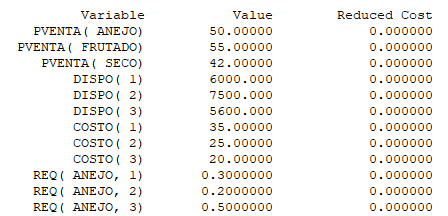
\includegraphics[width=0.95\textwidth]{fotos/eje7.png}
\end{center}

\newpage
\section{EJERCICIO 8: Prog Lineal con Solver: Extractos}

Se planteó un modelo de programación lineal para maximizar las ganancias en la producción de dos tipos de extractos: para beber y concentrado. El modelo fue resuelto utilizando el complemento \textbf{Solver de Excel}, obteniéndose una solución óptima.

\subsection{Función objetivo}
Maximizar:
\[
Z = 100X_1 + 200X_2
\]
donde:
\begin{itemize}
    \item \( X_1 \): hectolitros de extracto para beber
    \item \( X_2 \): hectolitros de extracto concentrado
\end{itemize}

\subsection{Restricciones}
\begin{align*}
300X_1 + 400X_2 &\leq 60000 && \text{(Fruta disponible)} \\
300X_1 + 200X_2 &\leq 48000 && \text{(Preservante)} \\
X_1 + 3X_2 &\geq 210 && \text{(Horas de trabajo)} \\
X_2 &\leq 2X_1 && \text{(Límite de proporción)} \\
X_1, X_2 &\geq 0 && \text{(No negatividad)}
\end{align*}

\subsection{Parámetros del problema}

\begin{table}
\centering
\begin{tabular}{lcccc}
\toprule
\textbf{Producto} & \textbf{Fruta (kg)} & \textbf{T. Trabajo (h)} & \textbf{Preservante (g)} & \textbf{Costo (\$)} \\
\midrule
Para beber        & 300                 & 1                       & 300                      & 100                \\
Concentrado       & 400                 & 3                       & 200                      & 200                \\
\bottomrule
\end{tabular}
\end{table}

\subsection{Disponibilidad de recursos}

\begin{itemize}
    \item Fruta: 60,000 kg
    \item Tiempo de trabajo: 210 horas (mínimo)
    \item Preservante: 48,000 gramos
\end{itemize}

\subsection{Resultados óptimos}

Los valores óptimos obtenidos con Solver fueron:

\begin{itemize}
    \item \( X_1 = 68.571 \) hectolitros de extracto para beber
    \item \( X_2 = 98.571 \) hectolitros de extracto concentrado
    \item \textbf{Ganancia total:} \$26,571.43
\end{itemize}

\subsection{Verificación de restricciones}

\begin{itemize}
    \item Fruta utilizada: \( 300(68.571) + 400(98.571) = 60000 \leq 60000 \)
    \item Preservante utilizado: \( 300(68.571) + 200(98.571) = 40285.71 \leq 48000 \)
    \item Horas trabajadas: \( 1(68.571) + 3(98.571) = 364.29 \geq 210 \)
    \item Proporción: \( X_2 = 98.571 \leq 2 \cdot 68.571 = 137.14 \)
\end{itemize}

\subsection{Interpretación}

\begin{itemize}
    \item La solución hace uso completo de la fruta disponible (60,000 kg).
    \item Se usa menos del total disponible de preservante (40,286 de 48,000 gramos).
    \item La exigencia mínima de 210 horas se supera ampliamente (364.29 h).
    \item La producción de extracto concentrado no excede el doble del extracto para beber.
    \item La ganancia máxima alcanzada es de \$26,571.43, distribuyendo eficientemente los recursos.
\end{itemize}


\newpage
\section{EJERCICIO 9:Prog Lineal Entera Asignación de Docentes}

\subsection{Planteamiento del problema}

La directora de un centro educativo desea asignar 5 asignaturas \( A1, A2, A3, A4, A5 \) a 4 profesores \( P1, P2, P3, P4 \) en base a valoraciones dadas por los alumnos. Además, hay restricciones:
\begin{itemize}
    \item El profesor P3 no puede impartir A1 ni A2.
    \item Cada asignatura debe ser impartida por un solo profesor.
    \item Ningún profesor puede tener más de 2 asignaturas.
    \item El profesor P1 sólo puede tener 1 asignatura.
\end{itemize}
El objetivo es maximizar la valoración total.

\subsection{Valoraciones promedio}

\begin{center}
\begin{tabular}{cccccc}
\toprule
 & A1 & A2 & A3 & A4 & A5 \\
\midrule
P1 & 2.7 & 2.2 & 3.4 & 2.8 & 3.8 \\
P2 & 3.6 & 3.4 & 2.8 & 3.6 & 3.5 \\
P3 & --  & --  & 3.1 & 2.9 & 3.3 \\
P4 & 2.6 & 2.5 & 1.8 & 4.2 & 3.5 \\
\bottomrule
\end{tabular}
\end{center}

\subsection{Función Objetivo}

Definimos variables binarias:
\[
x_{ij} =
\begin{cases}
1 & \text{si el profesor } i \text{ imparte la asignatura } j \\
0 & \text{en caso contrario}
\end{cases}
\]

Maximizar:
\[
Z = 2.7x_{11} + 2.2x_{12} + 3.4x_{13} + 2.8x_{14} + 3.8x_{15} + 3.6x_{21} + 3.4x_{22} + 2.8x_{23} + 3.6x_{24} + 3.5x_{25} + 3.1x_{33} + 2.9x_{34} + 3.3x_{35} + 2.6x_{41} + 2.5x_{42} + 1.8x_{43} + 4.2x_{44} + 3.5x_{45}
\]

\subsection{Restricciones}

\begin{itemize}
  \item Cada asignatura debe ser asignada a un solo profesor:
  \[
  \sum_{i=1}^4 x_{ij} = 1 \quad \forall j = 1,\ldots,5
  \]

  \item P1 puede tener máximo 1 asignatura:
  \[
  \sum_{j=1}^5 x_{1j} \leq 1
  \]

  \item P2, P3, P4 pueden tener máximo 2 asignaturas:
  \[
  \sum_{j=1}^5 x_{ij} \leq 2 \quad \forall i = 2,3,4
  \]

  \item P3 no puede impartir A1 ni A2:
  \[
  x_{31} = 0, \quad x_{32} = 0
  \]

  \item Variables binarias:
  \[
  x_{ij} \in \{0,1\}
  \]
\end{itemize}

\subsection{Solución}

Resolviendo con programación lineal entera, se obtiene la siguiente asignación óptima:

\begin{center}
\begin{tabular}{cc}
\toprule
Asignatura & Profesor Asignado \\
\midrule
A1 & P2 \\
A2 & P2 \\
A3 & P1 \\
A4 & P4 \\
A5 & P3 \\
\bottomrule
\end{tabular}
\end{center}

Valoración total máxima: \textbf{17.2}

\subsection{Conclusión}

La asignación óptima permite maximizar la valoración global respetando las restricciones del reglamento y de capacidad docente. Este tipo de modelado es muy útil en decisiones de planificación escolar.




\newpage
\section{Ejercicio 10: Prog Lineal :Compras e Inventarios}

\subsection{Planteamiento del problema}
Jack Biensaulk está encargado de comprar artículos enlatados para el servicio de alimentos de una universidad. Conoce la demanda mensual durante el año académico y los precios de compra. Puede adelantar compras para evitar alzas de precios, pero eso implica un costo de inventario de \$0.20 por caja al final de cada mes. No puede comprar más de 1500 cajas por mes. El objetivo es minimizar el costo total (compra e inventario).

\subsection{Función Objetivo}
Minimizar el costo total de compras e inventario:

\[
\min Z = \sum_{i=1}^{9} (Costo_i \cdot X_i + 0.2 \cdot Y_i)
\]

Donde:
\begin{itemize}
  \item \(X_i\): Cajas compradas en el mes \(i\)
  \item \(Y_i\): Cajas almacenadas al final del mes \(i\)
\end{itemize}

\subsection{Restricciones}

\begin{itemize}
  \item Capacidad máxima de compra mensual:
    \[
    X_i \leq 1500 \quad \forall i = 1,\ldots,9
    \]

  \item Balance de inventario:
  \begin{align*}
    Y_1 &= X_1 - Demanda_1 \\
    Y_i &= Y_{i-1} + X_i - Demanda_i \quad \forall i = 2,\ldots,9
  \end{align*}

  \item No negatividad:
  \[
  X_i \geq 0, \quad Y_i \geq 0
  \]
\end{itemize}

\subsection{Solución}

Luego de aplicar un modelo de programación lineal con software de optimización, se obtiene la siguiente solución óptima:

\begin{center}
\begin{tabular}{cccc}
\toprule
Mes & \(X_i\) (Compras) & \(Y_i\) (Inventario final) & Costo mensual (\$) \\
\midrule
1 & 1500 & 500 & 310.00 \\
2 & 900  & 500 & 190.00 \\
3 & 850  & 500 & 190.00 \\
4 & 1000 & 1000 & 430.00 \\
5 & 500  & 500 & 205.00 \\
6 & 1100 & 1000 & 455.00 \\
7 & 1000 & 1000 & 460.00 \\
8 & 500  & 300 & 204.00 \\
9 & 1200 & 300 & 474.00 \\
\bottomrule
\end{tabular}
\end{center}

Costo total aproximado: \textbf{\$2,918.00}

\subsection{Conclusión}
La estrategia óptima consiste en adelantar compras cuando los precios son más bajos y manejar adecuadamente el inventario para satisfacer la demanda futura, manteniéndose dentro del límite de compra mensual y minimizando el costo total del sistema.

\chapter{FUNCIONES MATEMATICAS}

\section{Definición de Función}

\begin{definicion}
Una \textbf{función} es una relación entre dos conjuntos, llamados dominio y codominio, que asigna a cada elemento del dominio exactamente un elemento del codominio.

Formalmente, una función $f: A \rightarrow B$ es una regla que asocia a cada elemento $x \in A$ un único elemento $y \in B$, denotado como $y = f(x)$.
\end{definicion}

\subsection{Elementos de una Función}

\begin{itemize}
    \item \textbf{Dominio ($Dom(f)$)}: Conjunto de todos los valores de entrada para los cuales la función está definida.
    \item \textbf{Codominio}: Conjunto al cual pertenecen todos los posibles valores de salida.
    \item \textbf{Rango o Imagen ($Im(f)$)}: Conjunto de todos los valores de salida que efectivamente toma la función.
    \item \textbf{Variable independiente}: La variable de entrada, usualmente denotada como $x$.
    \item \textbf{Variable dependiente}: La variable de salida, usualmente denotada como $y$ o $f(x)$.
\end{itemize}

\subsection{Notación y Representación}

Las funciones pueden representarse de diversas formas:

\subsection{Notación Algebraica}
$f(x) = x^2 + 2x - 1$

\subsection{Notación por Conjuntos}
$f = \{(x,y) \in \mathbb{R} \times \mathbb{R} : y = x^2 + 2x - 1\}$

\subsection{Tabla de Valores}
\begin{center}
\begin{tabular}{|c|c|}
\hline
$x$ & $f(x)$ \\
\hline
-2 & -1 \\
-1 & -2 \\
0 & -1 \\
1 & 2 \\
2 & 7 \\
\hline
\end{tabular}
\end{center}

\section{Clasificación de Funciones}

\subsection{Según su Forma Algebraica}

\subsection{Funciones Polinómicas}

\begin{definicion}
Una función polinómica es de la forma:
$f(x) = a_n x^n + a_{n-1} x^{n-1} + \cdots + a_1 x + a_0$
donde $a_i \in \mathbb{R}$ para $i = 0, 1, 2, \ldots, n$ y $a_n \neq 0$.
\end{definicion}

\subsubsection{Función Constante}
$f(x) = c \text{ donde } c \in \mathbb{R}$

\subsubsection{Función Lineal}
$f(x) = mx + b \text{ donde } m, b \in \mathbb{R} \text{ y } m \neq 0$

\subsubsection{Función Cuadrática}
$f(x) = ax^2 + bx + c \text{ donde } a, b, c \in \mathbb{R} \text{ y } a \neq 0$

\subsection{Funciones Racionales}

\begin{definicion}
Una función racional es el cociente de dos polinomios:
$f(x) = \frac{P(x)}{Q(x)}$
donde $P(x)$ y $Q(x)$ son polinomios y $Q(x) \neq 0$.
\end{definicion}

\subsection{Funciones Irracionales}

\begin{definicion}
Una función irracional contiene la variable independiente bajo un radical:
$f(x) = \sqrt[n]{g(x)}$
donde $g(x)$ es una expresión algebraica.
\end{definicion}

\subsection{Funciones Trascendentes}

\subsubsection{Funciones Exponenciales}
$f(x) = a^x \text{ donde } a > 0 \text{ y } a \neq 1$

\subsubsection{Funciones Logarítmicas}
$f(x) = \log_a(x) \text{ donde } a > 0, a \neq 1 \text{ y } x > 0$

\subsubsection{Funciones Trigonométricas}
\begin{align}
f(x) &= \sin(x) \\
f(x) &= \cos(x) \\
f(x) &= \tan(x)
\end{align}

\subsection{Según sus Propiedades}

\subsubsection{Funciones Inyectivas (Uno a Uno)}

\begin{definicion}
Una función $f: A \rightarrow B$ es inyectiva si:
$\forall x_1, x_2 \in A: x_1 \neq x_2 \Rightarrow f(x_1) \neq f(x_2)$
\end{definicion}

\subsubsection{Funciones Sobreyectivas (Sobre)}

\begin{definicion}
Una función $f: A \rightarrow B$ es sobreyectiva si:
$\forall y \in B, \exists x \in A \text{ tal que } f(x) = y$
\end{definicion}

\subsubsection{Funciones Biyectivas}

\begin{definicion}
Una función es biyectiva si es tanto inyectiva como sobreyectiva.
\end{definicion}

\subsubsection{Funciones Pares e Impares}

\begin{definicion}
\begin{itemize}
    \item Una función $f$ es \textbf{par} si $f(-x) = f(x)$ para todo $x$ en el dominio.
    \item Una función $f$ es \textbf{impar} si $f(-x) = -f(x)$ para todo $x$ en el dominio.
\end{itemize}
\end{definicion}

\subsubsection{Funciones Crecientes y Decrecientes}

\begin{definicion}
Sea $f$ una función definida en un intervalo $I$:
\begin{itemize}
    \item $f$ es \textbf{creciente} en $I$ si $x_1 < x_2 \Rightarrow f(x_1) \leq f(x_2)$
    \item $f$ es \textbf{estrictamente creciente} en $I$ si $x_1 < x_2 \Rightarrow f(x_1) < f(x_2)$
    \item $f$ es \textbf{decreciente} en $I$ si $x_1 < x_2 \Rightarrow f(x_1) \geq f(x_2)$
    \item $f$ es \textbf{estrictamente decreciente} en $I$ si $x_1 < x_2 \Rightarrow f(x_1) > f(x_2)$
\end{itemize}
\end{definicion}

\subsection{Operaciones con Funciones}

\subsection{Operaciones Algebraicas}

Sean $f$ y $g$ dos funciones con dominios $D_f$ y $D_g$ respectivamente.

\subsubsection{Suma de Funciones}
$(f + g)(x) = f(x) + g(x)$
Dominio: $D_{f+g} = D_f \cap D_g$

\subsubsection{Resta de Funciones}
$(f - g)(x) = f(x) - g(x)$
Dominio: $D_{f-g} = D_f \cap D_g$

\subsubsection{Producto de Funciones}
$(f \cdot g)(x) = f(x) \cdot g(x)$
Dominio: $D_{f \cdot g} = D_f \cap D_g$

\subsubsection{Cociente de Funciones}
$\left(\frac{f}{g}\right)(x) = \frac{f(x)}{g(x)}$
Dominio: $D_{f/g} = \{x \in D_f \cap D_g : g(x) \neq 0\}$

\subsection{Composición de Funciones}

\begin{definicion}
La composición de dos funciones $f$ y $g$, denotada como $(f \circ g)(x)$, se define como:
$(f \circ g)(x) = f(g(x))$
\end{definicion}

El dominio de $f \circ g$ es:
$D_{f \circ g} = \{x \in D_g : g(x) \in D_f\}$

\subsubsection{Propiedades de la Composición}

\begin{proposicion}
La composición de funciones es asociativa:
$(f \circ g) \circ h = f \circ (g \circ h)$
\end{proposicion}

\begin{proposicion}
La composición de funciones no es conmutativa en general:
$f \circ g \neq g \circ f$
\end{proposicion}

\subsection{Función Inversa}

\begin{definicion}
Sea $f: A \rightarrow B$ una función biyectiva. La función inversa de $f$, denotada como $f^{-1}: B \rightarrow A$, se define como:
$f^{-1}(y) = x \Leftrightarrow f(x) = y$
\end{definicion}

\subsubsection{Propiedades de la Función Inversa}

\begin{proposicion}
Si $f$ tiene inversa, entonces:
\begin{enumerate}
    \item $(f^{-1})^{-1} = f$
    \item $f \circ f^{-1} = I_B$ (función identidad en $B$)
    \item $f^{-1} \circ f = I_A$ (función identidad en $A$)
\end{enumerate}
\end{proposicion}

\subsection{Límites y Continuidad}

\subsection{Concepto de Límite}

\begin{definicion}
El límite de una función $f(x)$ cuando $x$ tiende a $a$ es $L$, denotado como:
$\lim_{x \to a} f(x) = L$
si para todo $\varepsilon > 0$, existe un $\delta > 0$ tal que:
$0 < |x - a| < \delta \Rightarrow |f(x) - L| < \varepsilon$
\end{definicion}

\subsubsection{Propiedades de los Límites}

Si $\lim_{x \to a} f(x) = L$ y $\lim_{x \to a} g(x) = M$, entonces:

\begin{enumerate}
    \item $\lim_{x \to a} [f(x) + g(x)] = L + M$
    \item $\lim_{x \to a} [f(x) - g(x)] = L - M$
    \item $\lim_{x \to a} [f(x) \cdot g(x)] = L \cdot M$
    \item $\lim_{x \to a} \frac{f(x)}{g(x)} = \frac{L}{M}$ (si $M \neq 0$)
    \item $\lim_{x \to a} [c \cdot f(x)] = c \cdot L$ (donde $c$ es constante)
\end{enumerate}

\subsection{Continuidad}

\begin{definicion}
Una función $f$ es continua en $x = a$ si:
\begin{enumerate}
    \item $f(a)$ está definida
    \item $\lim_{x \to a} f(x)$ existe
    \item $\lim_{x \to a} f(x) = f(a)$
\end{enumerate}
\end{definicion}

\subsubsection{Tipos de Discontinuidades}

\begin{enumerate}
    \item \textbf{Discontinuidad evitable}: El límite existe pero no es igual al valor de la función en ese punto.
    \item \textbf{Discontinuidad de salto}: Los límites laterales existen pero son diferentes.
    \item \textbf{Discontinuidad esencial}: Al menos uno de los límites laterales no existe.
\end{enumerate}

\subsection{Derivadas de Funciones}

\subsection{Definición de Derivada}

\begin{definicion}
La derivada de una función $f$ en el punto $x = a$ se define como:
$f'(a) = \lim_{h \to 0} \frac{f(a + h) - f(a)}{h}$
siempre que este límite exista.
\end{definicion}

\subsubsection{Interpretación Geométrica}

La derivada de una función en un punto representa la pendiente de la recta tangente a la curva en ese punto.

\subsubsection{Interpretación Física}

En el contexto físico, la derivada representa la tasa instantánea de cambio de una cantidad con respecto a otra.

\subsection{Reglas de Derivación}

\subsubsection{Reglas Básicas}

\begin{enumerate}
    \item \textbf{Regla de la constante}: $\frac{d}{dx}[c] = 0$
    \item \textbf{Regla de la potencia}: $\frac{d}{dx}[x^n] = nx^{n-1}$
    \item \textbf{Regla del múltiplo constante}: $\frac{d}{dx}[cf(x)] = c \cdot f'(x)$
    \item \textbf{Regla de la suma}: $\frac{d}{dx}[f(x) + g(x)] = f'(x) + g'(x)$
    \item \textbf{Regla del producto}: $\frac{d}{dx}[f(x) \cdot g(x)] = f'(x) \cdot g(x) + f(x) \cdot g'(x)$
    \item \textbf{Regla del cociente}: $\frac{d}{dx}\left[\frac{f(x)}{g(x)}\right] = \frac{f'(x) \cdot g(x) - f(x) \cdot g'(x)}{[g(x)]^2}$
\end{enumerate}

\subsubsection{Regla de la Cadena}

\begin{teorema}
Si $y = f(u)$ y $u = g(x)$, entonces:
$\frac{dy}{dx} = \frac{dy}{du} \cdot \frac{du}{dx} = f'(u) \cdot g'(x) = f'(g(x)) \cdot g'(x)$
\end{teorema}

\subsection{Derivadas de Funciones Especiales}

\subsubsection{Funciones Trigonométricas}
\begin{align}
\frac{d}{dx}[\sin x] &= \cos x \\
\frac{d}{dx}[\cos x] &= -\sin x \\
\frac{d}{dx}[\tan x] &= \sec^2 x
\end{align}

\subsection{Funciones Exponenciales y Logarítmicas}
\begin{align}
\frac{d}{dx}[e^x] &= e^x \\
\frac{d}{dx}[a^x] &= a^x \ln a \\
\frac{d}{dx}[\ln x] &= \frac{1}{x} \\
\frac{d}{dx}[\log_a x] &= \frac{1}{x \ln a}
\end{align}

\subsection{Integrales de Funciones}

\subsection{Integral Indefinida}

\begin{definicion}
La integral indefinida de una función $f(x)$ es una función $F(x)$ tal que $F'(x) = f(x)$. Se denota como:
$\int f(x) \, dx = F(x) + C$
donde $C$ es la constante de integración.
\end{definicion}

\subsubsection{Propiedades de la Integral Indefinida}

\begin{enumerate}
    \item $\int [f(x) + g(x)] \, dx = \int f(x) \, dx + \int g(x) \, dx$
    \item $\int c \cdot f(x) \, dx = c \int f(x) \, dx$
    \item $\int x^n \, dx = \frac{x^{n+1}}{n+1} + C$ (para $n \neq -1$)
    \item $\int \frac{1}{x} \, dx = \ln|x| + C$
    \item $\int e^x \, dx = e^x + C$
\end{enumerate}

\subsection{Integral Definida}

\begin{definicion}
La integral definida de una función $f(x)$ desde $x = a$ hasta $x = b$ se define como:
$\int_a^b f(x) \, dx = \lim_{n \to \infty} \sum_{i=1}^n f(x_i) \Delta x$
donde $\Delta x = \frac{b-a}{n}$ y $x_i = a + i \cdot \Delta x$.
\end{definicion}

\subsubsection{Teorema Fundamental del Cálculo}

\begin{teorema}
Si $f$ es continua en $[a,b]$ y $F$ es una antiderivada de $f$, entonces:
$\int_a^b f(x) \, dx = F(b) - F(a)$
\end{teorema}

\section{Ejercicios Resueltos}

\begin{ejercicio}
\textbf{Ejercicio 1: Función Cuadrática}

Dada la función $f(x) = x^2 - 4x + 3$, determinar:
\begin{enumerate}[label=\alph*)]
    \item El dominio y rango de la función
    \item Los ceros de la función
    \item El vértice de la parábola
    \item La ecuación del eje de simetría
\end{enumerate}
\end{ejercicio}

\textbf{Solución:}

a) \textbf{Dominio y Rango:}
\begin{itemize}
    \item Dominio: $Dom(f) = \mathbb{R}$ (toda función cuadrática está definida para todos los números reales)
    \item Para el rango, completamos el cuadrado:
    $f(x) = x^2 - 4x + 3 = (x-2)^2 - 4 + 3 = (x-2)^2 - 1$
    \item Como $(x-2)^2 \geq 0$, tenemos $f(x) \geq -1$
    \item Rango: $Ran(f) = [-1, +\infty)$
\end{itemize}

b) \textbf{Ceros de la función:}
Resolvemos $f(x) = 0$:
$x^2 - 4x + 3 = 0$
Factorizando: $(x-1)(x-3) = 0$
Por lo tanto: $x = 1$ o $x = 3$

c) \textbf{Vértice de la parábola:}
De la forma canónica $f(x) = (x-2)^2 - 1$, el vértice es $(2, -1)$

d) \textbf{Eje de simetría:}
La ecuación del eje de simetría es $x = 2$

\begin{ejercicio}
\textbf{Ejercicio 2: Función Racional}

Analizar la función $g(x) = \frac{2x + 1}{x - 3}$:
\begin{enumerate}[label=\alph*)]
    \item Determinar el dominio
    \item Encontrar las asíntotas
    \item Calcular los puntos de intersección con los ejes
\end{enumerate}
\end{ejercicio}

\textbf{Solución:}

a) \textbf{Dominio:}
La función está definida para todos los valores de $x$ excepto donde el denominador es cero:
$x - 3 = 0 \Rightarrow x = 3$
Dominio: $Dom(g) = \mathbb{R} \setminus \{3\} = (-\infty, 3) \cup (3, +\infty)$

b) \textbf{Asíntotas:}
\begin{itemize}
    \item \textbf{Asíntota vertical:} $x = 3$ (donde el denominador se anula)
    \item \textbf{Asíntota horizontal:} Como el grado del numerador igual al del denominador:
    $y = \frac{2}{1} = 2$
\end{itemize}

c) \textbf{Intersecciones con los ejes:}
\begin{itemize}
    \item \textbf{Con el eje y:} $g(0) = \frac{2(0) + 1}{0 - 3} = \frac{1}{-3} = -\frac{1}{3}$. Punto: $(0, -\frac{1}{3})$
    \item \textbf{Con el eje x:} $g(x) = 0 \Rightarrow 2x + 1 = 0 \Rightarrow x = -\frac{1}{2}$. Punto: $(-\frac{1}{2}, 0)$
\end{itemize}

\begin{ejercicio}
\textbf{Ejercicio 3: Composición de Funciones}

Sean $f(x) = x^2 + 1$ y $g(x) = 2x - 3$. Calcular:
\begin{enumerate}[label=\alph*)]
    \item $(f \circ g)(x)$
    \item $(g \circ f)(x)$
    \item $(f \circ g)(2)$
    \item $(g \circ f)(-1)$
\end{enumerate}
\end{ejercicio}

\textbf{Solución:}

a) \textbf{$(f \circ g)(x) = f(g(x))$:}
$f(g(x)) = f(2x - 3) = (2x - 3)^2 + 1$
$= 4x^2 - 12x + 9 + 1 = 4x^2 - 12x + 10$

b) \textbf{$(g \circ f)(x) = g(f(x))$:}
$g(f(x)) = g(x^2 + 1) = 2(x^2 + 1) - 3$
$= 2x^2 + 2 - 3 = 2x^2 - 1$

c) \textbf{$(f \circ g)(2)$:}
$(f \circ g)(2) = 4(2)^2 - 12(2) + 10 = 16 - 24 + 10 = 2$

d) \textbf{$(g \circ f)(-1)$:}
$(g \circ f)(-1) = 2(-1)^2 - 1 = 2(1) - 1 = 1$

\begin{ejercicio}
\textbf{Ejercicio 4: Función Exponencial}

Para la función $h(x) = 3 \cdot 2^{x-1} + 4$:
\begin{enumerate}[label=\alph*)]
    \item Determinar el dominio y rango
    \item Encontrar la asíntota horizontal
    \item Calcular $h(0)$, $h(1)$, y $h(3)$
    \item Resolver $h(x) = 16$
\end{enumerate}
\end{ejercicio}

\textbf{Solución:}

a) \textbf{Dominio y Rango:}
\begin{itemize}
    \item Dominio: $Dom(h) = \mathbb{R}$ (las funciones exponenciales están definidas para todos los reales)
    \item Como $2^{x-1} > 0$ para todo $x$, tenemos $3 \cdot 2^{x-1} > 0$
    \item Por lo tanto: $h(x) = 3 \cdot 2^{x-1} + 4 > 4$
    \item Rango: $Ran(h) = (4, +\infty)$
\end{itemize}

b) \textbf{Asíntota horizontal:}
Cuando $x \to -\infty$: $2^{x-1} \to 0$, por lo tanto $h(x) \to 4$
Asíntota horizontal: $y = 4$

c) \textbf{Valores específicos:}
\begin{align}
h(0) &= 3 \cdot 2^{0-1} + 4 = 3 \cdot 2^{-1} + 4 = 3 \cdot \frac{1}{2} + 4 = \frac{3}{2} + 4 = \frac{11}{2} \\
h(1) &= 3 \cdot 2^{1-1} + 4 = 3 \cdot 2^0 + 4 = 3 \cdot 1 + 4 = 7 \\
h(3) &= 3 \cdot 2^{3-1} + 4 = 3 \cdot 2^2 + 4 = 3 \cdot 4 + 4 = 16
\end{align}

d) \textbf{Resolver $h(x) = 16$:}
$3 \cdot 2^{x-1} + 4 = 16$
$3 \cdot 2^{x-1} = 12$
$2^{x-1} = 4 = 2^2$
$x - 1 = 2$
$x = 3$

\begin{ejercicio}
\textbf{Ejercicio 5: Función Logarítmica}

Dada la función $k(x) = \log_2(x + 3) - 1$:
\begin{enumerate}[label=\alph*)]
    \item Determinar el dominio
    \item Encontrar las intersecciones con los ejes
    \item Hallar la asíntota vertical
    \item Resolver $k(x) = 2$
\end{enumerate}
\end{ejercicio}

\textbf{Solución:}

a) \textbf{Dominio:}
Para que el logaritmo esté definido: $x + 3 > 0 \Rightarrow x > -3$
Dominio: $Dom(k) = (-3, +\infty)$

b) \textbf{Intersecciones con los ejes:}
\begin{itemize}
    \item \textbf{Con el eje y:} $k(0) = \log_2(0 + 3) - 1 = \log_2(3) - 1 \approx 1.585 - 1 = 0.585$
    \item \textbf{Con el eje x:} $k(x) = 0$
    $\log_2(x + 3) - 1 = 0$
    $\log_2(x + 3) = 1$
    $x + 3 = 2^1 = 2$
    $x = -1$
    Punto: $(-1, 0)$
\end{itemize}

c) \textbf{Asíntota vertical:}
Cuando $x \to -3^+$: $x + 3 \to 0^+$, por lo tanto $\log_2(x + 3) \to -\infty$
Asíntota vertical: $x = -3$

d) \textbf{Resolver $k(x) = 2$:}
$\log_2(x + 3) - 1 = 2$
$\log_2(x + 3) = 3$
$x + 3 = 2^3 = 8$
$x = 5$

\begin{ejercicio}
\textbf{Ejercicio 6: Límites}

Calcular los siguientes límites:
\begin{enumerate}[label=\alph*)]
    \item $\lim_{x \to 2} \frac{x^2 - 4}{x - 2}$
    \item $\lim_{x \to 0} \frac{\sin x}{x}$
    \item $\lim_{x \to \infty} \frac{3x^2 + 2x - 1}{x^2 - 5x + 6}$
\end{enumerate}
\end{ejercicio}

\textbf{Solución:}

a) \textbf{$\lim_{x \to 2} \frac{x^2 - 4}{x - 2}$:}
Factorizamos el numerador:
$\lim_{x \to 2} \frac{x^2 - 4}{x - 2} = \lim_{x \to 2} \frac{(x-2)(x+2)}{x - 2}$
$= \lim_{x \to 2} (x + 2) = 2 + 2 = 4$

b) \textbf{$\lim_{x \to 0} \frac{\sin x}{x}$:}
Este es un límite fundamental:
$\lim_{x \to 0} \frac{\sin x}{x} = 1$

c) \textbf{$\lim_{x \to \infty} \frac{3x^2 + 2x - 1}{x^2 - 5x + 6}$:}
Dividimos numerador y denominador por $x^2$:
$\lim_{x \to \infty} \frac{3 + \frac{2}{x} - \frac{1}{x^2}}{1 - \frac{5}{x} + \frac{6}{x^2}} = \frac{3 + 0 - 0}{1 - 0 + 0} = 3$

\begin{ejercicio}
\textbf{Ejercicio 7: Derivadas}

Calcular las derivadas de las siguientes funciones:
\begin{enumerate}[label=\alph*)]
    \item $f(x) = x^3 - 2x^2 + 5x - 1$
    \item $g(x) = \frac{x^2 + 1}{x - 1}$
    \item $h(x) = e^{2x} \cos(3x)$
    \item $k(x) = \ln(x^2 + 1)$
\end{enumerate}
\end{ejercicio}

\textbf{Solución:}

a) \textbf{$f(x) = x^3 - 2x^2 + 5x - 1$:}
$f'(x) = 3x^2 - 4x + 5$

b) \textbf{$g(x) = \frac{x^2 + 1}{x - 1}$:}
Usando la regla del cociente:
$g'(x) = \frac{(2x)(x-1) - (x^2+1)(1)}{(x-1)^2}$
$= \frac{2x^2 - 2x - x^2 - 1}{(x-1)^2} = \frac{x^2 - 2x - 1}{(x-1)^2}$

c) \textbf{$h(x) = e^{2x} \cos(3x)$:}
Usando la regla del producto:
$h'(x) = 2e^{2x} \cos(3x) + e^{2x}(-3\sin(3x))$
$= e^{2x}[2\cos(3x) - 3\sin(3x)]$

d) \textbf{$k(x) = \ln(x^2 + 1)$:}
Usando la regla de la cadena:
$k'(x) = \frac{1}{x^2 + 1} \cdot 2x = \frac{2x}{x^2 + 1}$

\begin{ejercicio}
\textbf{Ejercicio 8: Integrales Indefinidas}

Calcular las siguientes integrales:
\begin{enumerate}[label=\alph*)]
    \item $\int (3x^2 - 2x + 1) \, dx$
    \item $\int \frac{1}{x^2 + 1} \, dx$
    \item $\int x e^x \, dx$
    \item $\int \frac{2x}{x^2 + 1} \, dx$
\end{enumerate}
\end{ejercicio}

\textbf{Solución:}

a) \textbf{$\int (3x^2 - 2x + 1) \, dx$:}
$\int (3x^2 - 2x + 1) \, dx = x^3 - x^2 + x + C$

b) \textbf{$\int \frac{1}{x^2 + 1} \, dx$:}
Esta es una integral estándar:
$\int \frac{1}{x^2 + 1} \, dx = \arctan(x) + C$

c) \textbf{$\int x e^x \, dx$:}
Usando integración por partes: $u = x$, $dv = e^x dx$
$\int x e^x \, dx = x e^x - \int e^x \, dx = x e^x - e^x + C = e^x(x - 1) + C$

d) \textbf{$\int \frac{2x}{x^2 + 1} \, dx$:}
Por sustitución: $u = x^2 + 1$, $du = 2x \, dx$
$\int \frac{2x}{x^2 + 1} \, dx = \int \frac{1}{u} \, du = \ln|u| + C = \ln(x^2 + 1) + C$

\begin{ejercicio}
\textbf{Ejercicio 9: Integrales Definidas}

Evaluar las siguientes integrales definidas:
\begin{enumerate}[label=\alph*)]
    \item $\int_0^2 (x^2 + 1) \, dx$
    \item $\int_1^e \frac{1}{x} \, dx$
    \item $\int_0^{\pi/2} \sin x \, dx$
\end{enumerate}
\end{ejercicio}

\textbf{Solución:}

a) \textbf{$\int_0^2 (x^2 + 1) \, dx$:}
$\int_0^2 (x^2 + 1) \, dx = \left[\frac{x^3}{3} + x\right]_0^2$
$= \left(\frac{8}{3} + 2\right) - (0 + 0) = \frac{8}{3} + 2 = \frac{14}{3}$

b) \textbf{$\int_1^e \frac{1}{x} \, dx$:}
$\int_1^e \frac{1}{x} \, dx = [\ln x]_1^e = \ln e - \ln 1 = 1 - 0 = 1$

c) \textbf{$\int_0^{\pi/2} \sin x \, dx$:}
$\int_0^{\pi/2} \sin x \, dx = [-\cos x]_0^{\pi/2}$
$= -\cos(\pi/2) - (-\cos 0) = -0 + 1 = 1$

\begin{ejercicio}
\textbf{Ejercicio 10: Problema de Aplicación}

Una partícula se mueve a lo largo de una línea recta. Su posición en el tiempo $t$ está dada por:
$s(t) = t^3 - 6t^2 + 9t + 2$
donde $s$ se mide en metros y $t$ en segundos.

\begin{enumerate}[label=\alph*)]
    \item Encontrar la velocidad $v(t)$ y la aceleración $a(t)$
    \item Determinar cuándo la partícula está en reposo
    \item Calcular la distancia total recorrida en los primeros 4 segundos
\end{enumerate}
\end{ejercicio}

\textbf{Solución:}

a) \textbf{Velocidad y aceleración:}
$v(t) = s'(t) = 3t^2 - 12t + 9$
$a(t) = v'(t) = 6t - 12$

b) \textbf{Partícula en reposo:}
La partícula está en reposo cuando $v(t) = 0$:
$3t^2 - 12t + 9 = 0$
$t^2 - 4t + 3 = 0$
$(t - 1)(t - 3) = 0$
Por lo tanto: $t = 1$ s y $t = 3$ s

c) \textbf{Distancia total recorrida:}
Primero evaluamos la posición en los puntos críticos:
\begin{align}
s(0) &= 0 - 0 + 0 + 2 = 2 \\
s(1) &= 1 - 6 + 9 + 2 = 6 \\
s(3) &= 27 - 54 + 27 + 2 = 2 \\
s(4) &= 64 - 96 + 36 + 2 = 6
\end{align}

La partícula se mueve:
- De $t = 0$ a $t = 1$: de posición 2 a 6 (distancia = 4 m)
- De $t = 1$ a $t = 3$: de posición 6 a 2 (distancia = 4 m)
- De $t = 3$ a $t = 4$: de posición 2 a 6 (distancia = 4 m)

Distancia total = $4 + 4 + 4 = 12$ metros

\section{Conclusiones}

Las funciones matemáticas constituyen uno de los pilares fundamentales del análisis matemático y tienen aplicaciones extensas en todas las ramas de la ciencia y la ingeniería. A través de este libro hemos explorado:

\begin{itemize}
    \item Los conceptos fundamentales de funciones y sus propiedades
    \item La clasificación de funciones según su forma algebraica y propiedades
    \item Las operaciones entre funciones, incluyendo la composición y la función inversa
    \item Los conceptos de límite y continuidad
    \item El cálculo diferencial y sus aplicaciones
    \item El cálculo integral y sus aplicaciones
\end{itemize}

Los ejercicios resueltos proporcionan ejemplos prácticos de cómo aplicar estos conceptos en situaciones concretas, desde problemas algebraicos básicos hasta aplicaciones en física y movimiento.

El dominio de estos conceptos es esencial para el estudio avanzado de matemáticas, física, ingeniería y muchas otras disciplinas científicas. Las funciones matemáticas nos permiten modelar fenómenos del mundo real y resolver problemas complejos mediante herramientas analíticas poderosas.

\end{document}